\chapter{Evaluation}
\newcommand{\rd}[1]{\textcolor{red}{#1}}
\newcommand{\gn}[1]{\textcolor{green}{#1}}

\label{Chapter5}

in the previous chapter \ref{Chapter4} the test bed implementation was introduced. In this chapter this test bed is used to evaluate the performance of the system proposed in chapter \ref{Chapter3}.

The evaluated components of the system are the room recognition and the room based weighting method for the transliteration.

Before presenting the evaluation results section \ref{TestBedDeployment} introduces the environment where the test bed was deployed and the data sets used for the evaluation. Sections \ref{EvaluationRoomRecognition} and \ref{EvaluationWeighting} then evaluate the room recognition and weighting.

\section{Test bed deployment and collected data sets}
\label{TestBedDeployment}

\begin{figure}[ht]
\centering
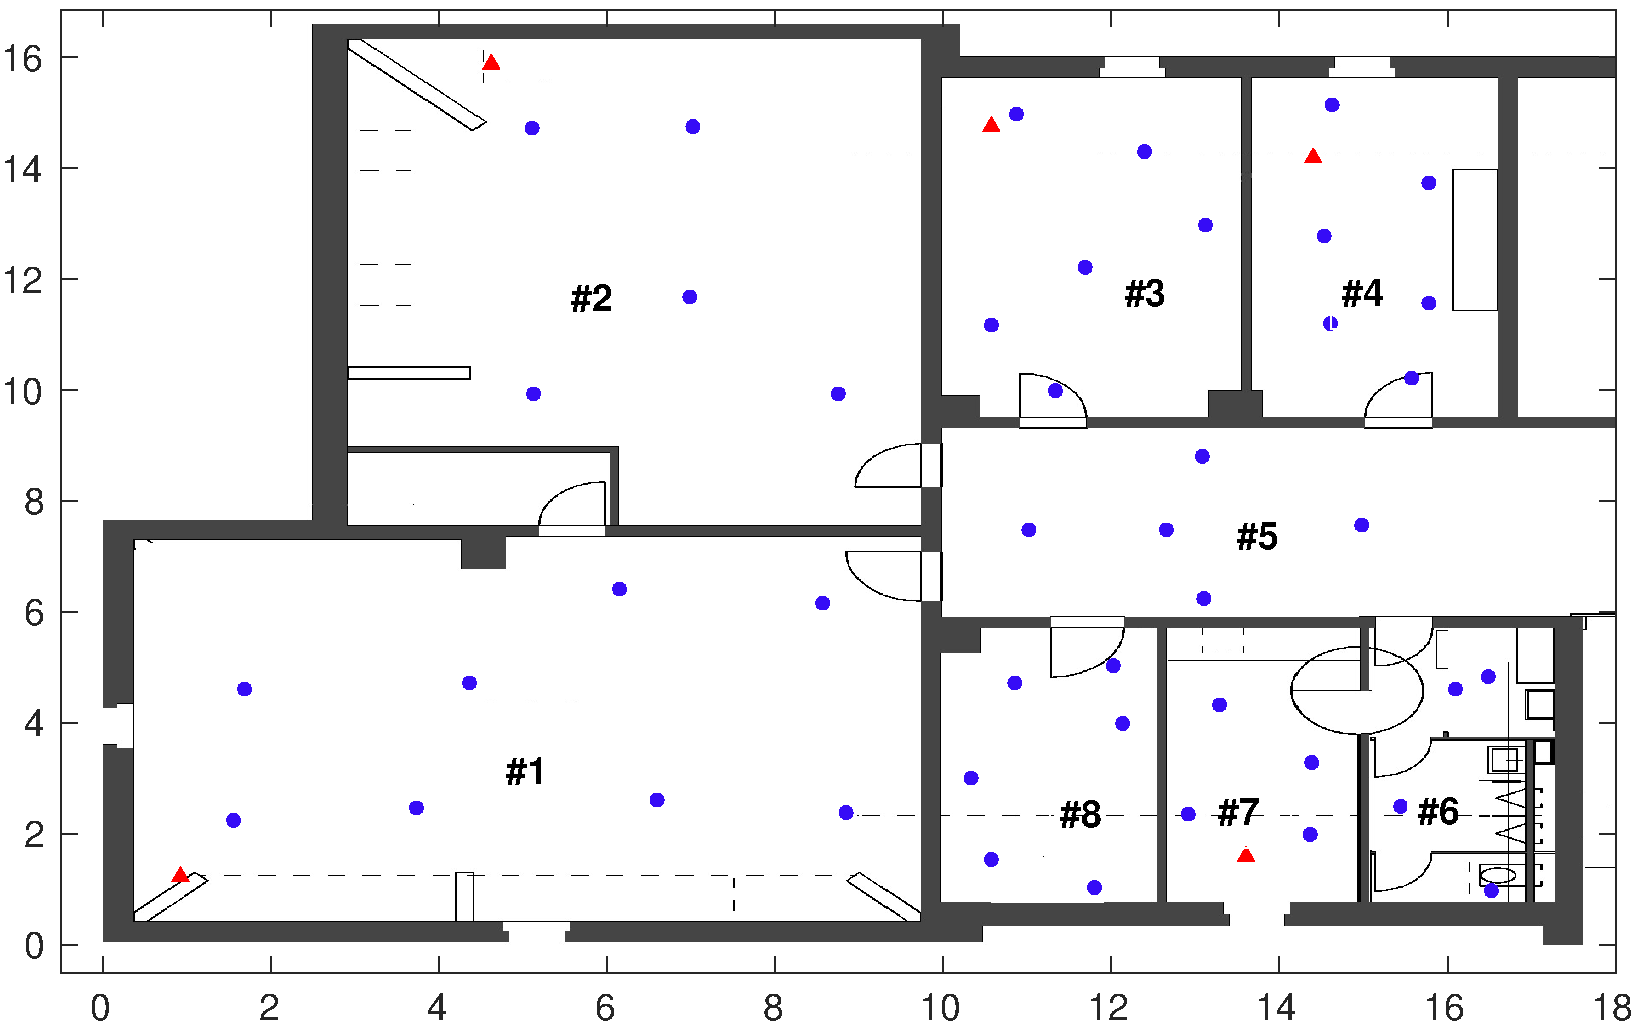
\includegraphics[width=\textwidth]{Figures/FloorPlan_ANs}
\decoRule
\caption[Floor plan with anchor node placement]{Floor plan showing the area of interest with the anchor nodes in red, the \emph{XY}-samples in blue and the room numbers in black}
\label{fig:FloorPlanANs}
\end{figure}

The test bed was deployed on the third floor at the Institute of Computer Science (INF) of the University of Bern. The area of interest is 297m\textsuperscript{2} in size, with seven rooms connected by a large corridor. The five anchor nodes were positioned to provide maximum coverage of the area so that the mobile node is able to receive at least four of the signals at all time. The rooms were given numbers form one to eight, the corridor being also treated as a room.

\subsection{Collected Data Sets}

The samples are collected with the smartphone held approximatively one meter above the ground and always pointing in the same cardinal direction. This is important because the magnetic field measurements are influenced by the devices orientation.

The collected samples were grouped into the following data sets:

\begin{itemize}
\item \textbf{Fingerprinting data} only labelled with the room number
	\begin{itemize}
	\item Grid (223 samples)

	A set of \textbf{evenly distributed} samples gathered in a grid pattern with approximately 1.2m distance between them.
	\item Borders (373 samples)
	
	A set of \textbf{unevenly distributed} samples. The sample density is very high at the borders (walls and doors between rooms) with about one sample taken every 0.5m but only a few samples from the center of each room.
	\end{itemize}
 \item \textbf{XY data} labelled with the exact coordinates
 
 A set of 44 \textbf{evenly distributed} samples with \((X,Y)\)-coordinates.
\end{itemize}

\section{Room Recognition}
\label{EvaluationRoomRecognition}

The purpose of this experiment is to check the hypothesis that the magnetic field data improves the room recognition accuracy and find out which kind of training data (evenly distributed or more samples at the borders) achieves the best results.

\paragraph{To check if the magnetic field data has a significant impact on the performance of the room recognition} 10-fold cross validation is performed on the evenly distributed \emph{Grid} data set both with and without using magnetic field data. The resulting accuracies are then compared. This experiment is repeated with different SVM parameters to see if the parameters have an impact on the result. 

\paragraph{To determine the best training data set} multiple models are generated using different training data, parameters and kernels and evaluated against the \emph{XY} data set.

The parameters are either the standard pre-sets or selected with cross validation and grid search. The training data used are the \emph{Grid}, \emph{Center} and \emph{Borders} data sets and a combination of the \emph{Borders} and \emph{Center} data set.

\subsection{Results}

Table \ref{tab:RoomRecognitionMagneticField} shows a large difference between the performance with and without magnetic field data. On average the accuracy was 26.8\% higher with the magnetic field data. For the paired students T-Test this results in a $t_{obs}$ of 13.0.The theoretical limit with a student's distribution and 9 degrees of freedom with a confidence level of 5\% is 2.262. The difference between the two sets of samples is therefore statistically significant.

\begin{table}
\centering
\begin{tabular}{l l l}
\toprule
\textbf{Sample}&\boldmath$RSSI_{i},B_{xyz}$&\boldmath$RSSI_{i}$ \\
\midrule
1&90\%&52.9\% \\
2&90.2\%&70.5\% \\
3&88.5\%&62.3\% \\
4&88.3\%&67.5\% \\
5&91.2\%&52.9\% \\
6&84.8\%&61.0\% \\
7&89.6\%&61.2\% \\
8&96.8\%&76.7\% \\
9&94.4\%&68.5\% \\
10&85.3\%&57.4\% \\
\textbf{Mean}&\textbf{89.9}&\textbf{63.1} \\
\bottomrule
\end{tabular}
\caption[Room Recognition - Magnetic Field]{Accuracy of the room recognition with and without magnetic field data.}
\label{tab:RoomRecognitionMagneticField}
\end{table}

\begin{table}
\centering
\begin{tabular}{l l l l}
\toprule
\textbf{Sample}&\boldmath$RSSI_{i},B_{xyz}$&\boldmath$RSSI_{i}$&\textbf{Difference} \\
\midrule
CV (pre-set)&90.1\%&70.4\%&19.7\%\\
CV (optimized)&93.3\%&83.0\%&10.3\%\\
XY test set&84.1\%&81.8\%&2.3\%\\
XY test set&97.3\%&86.8\%&10.5\%\\
\textit{(without room \#3)}&&\\
\bottomrule
\end{tabular}
\caption[Room Recognition - Magnetic Field]{Accuracy of the room recognition with and without magnetic field data.}
\label{tab:RoomRecognitionMagneticField}
\end{table}

\begin{figure}[ht]

\label{fig:FloorPlanRoomError}
\centering
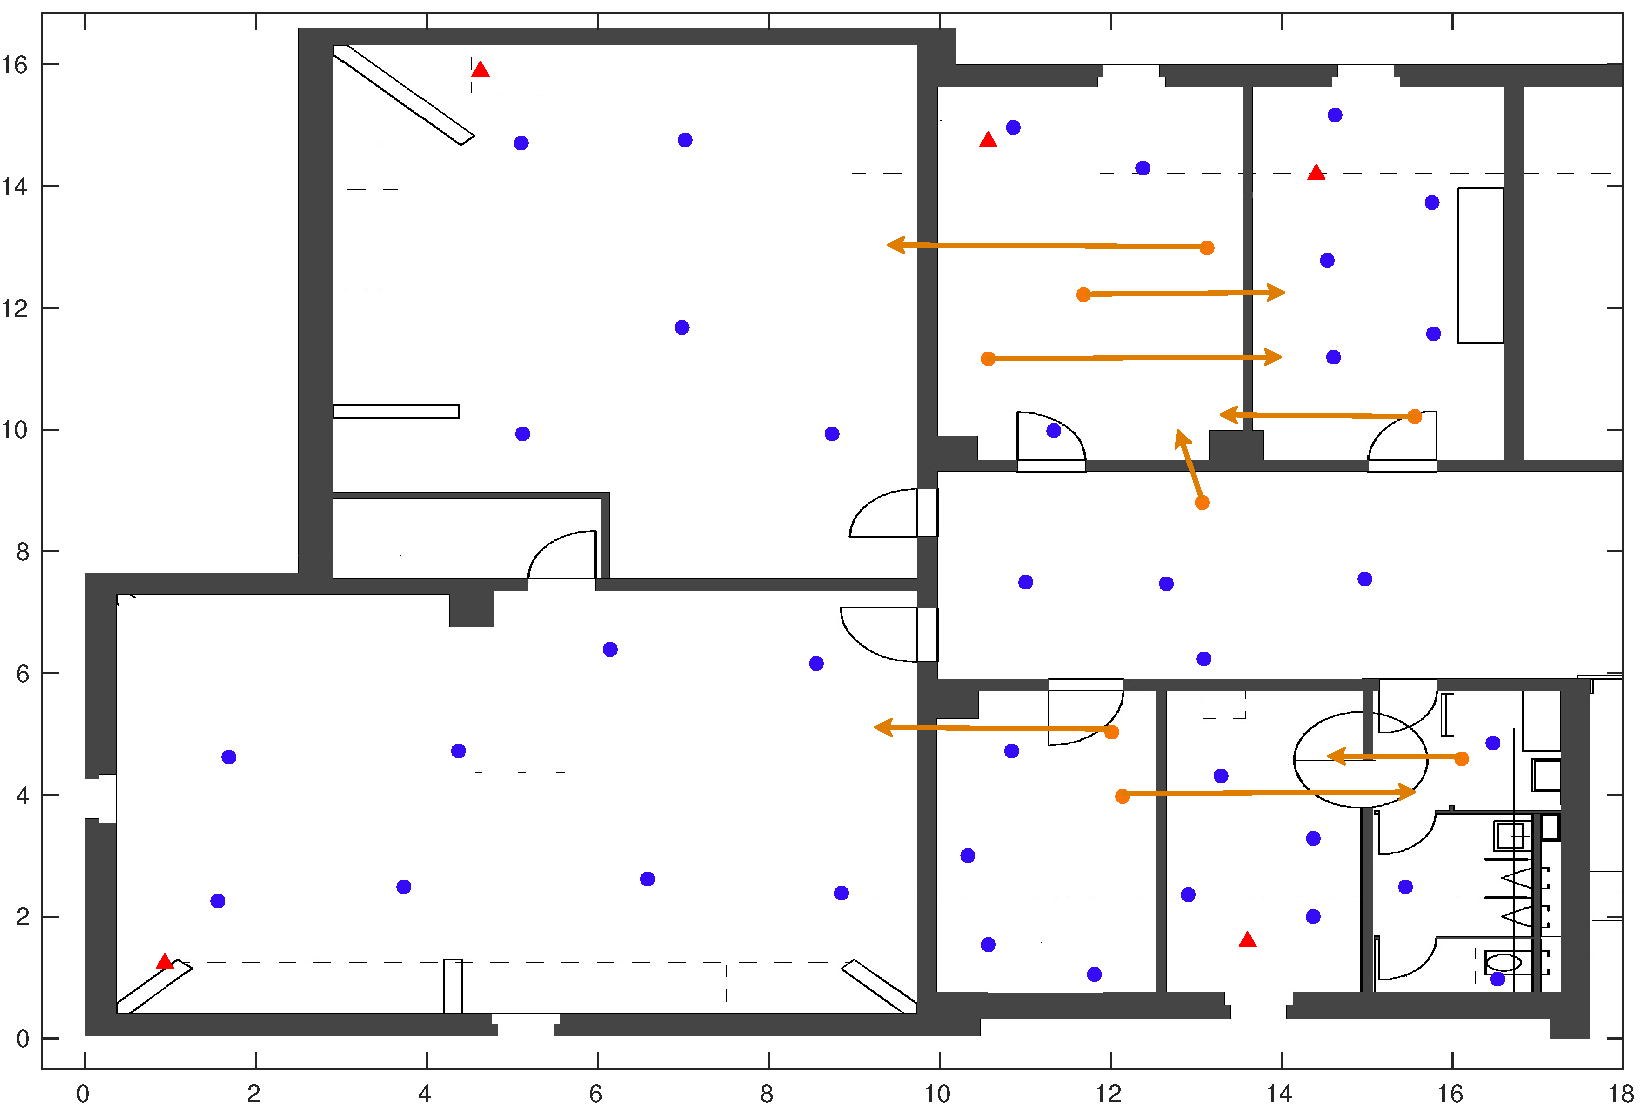
\includegraphics[width=.8\textwidth]{Figures/FloorPlan_Room_error_WO_MF}
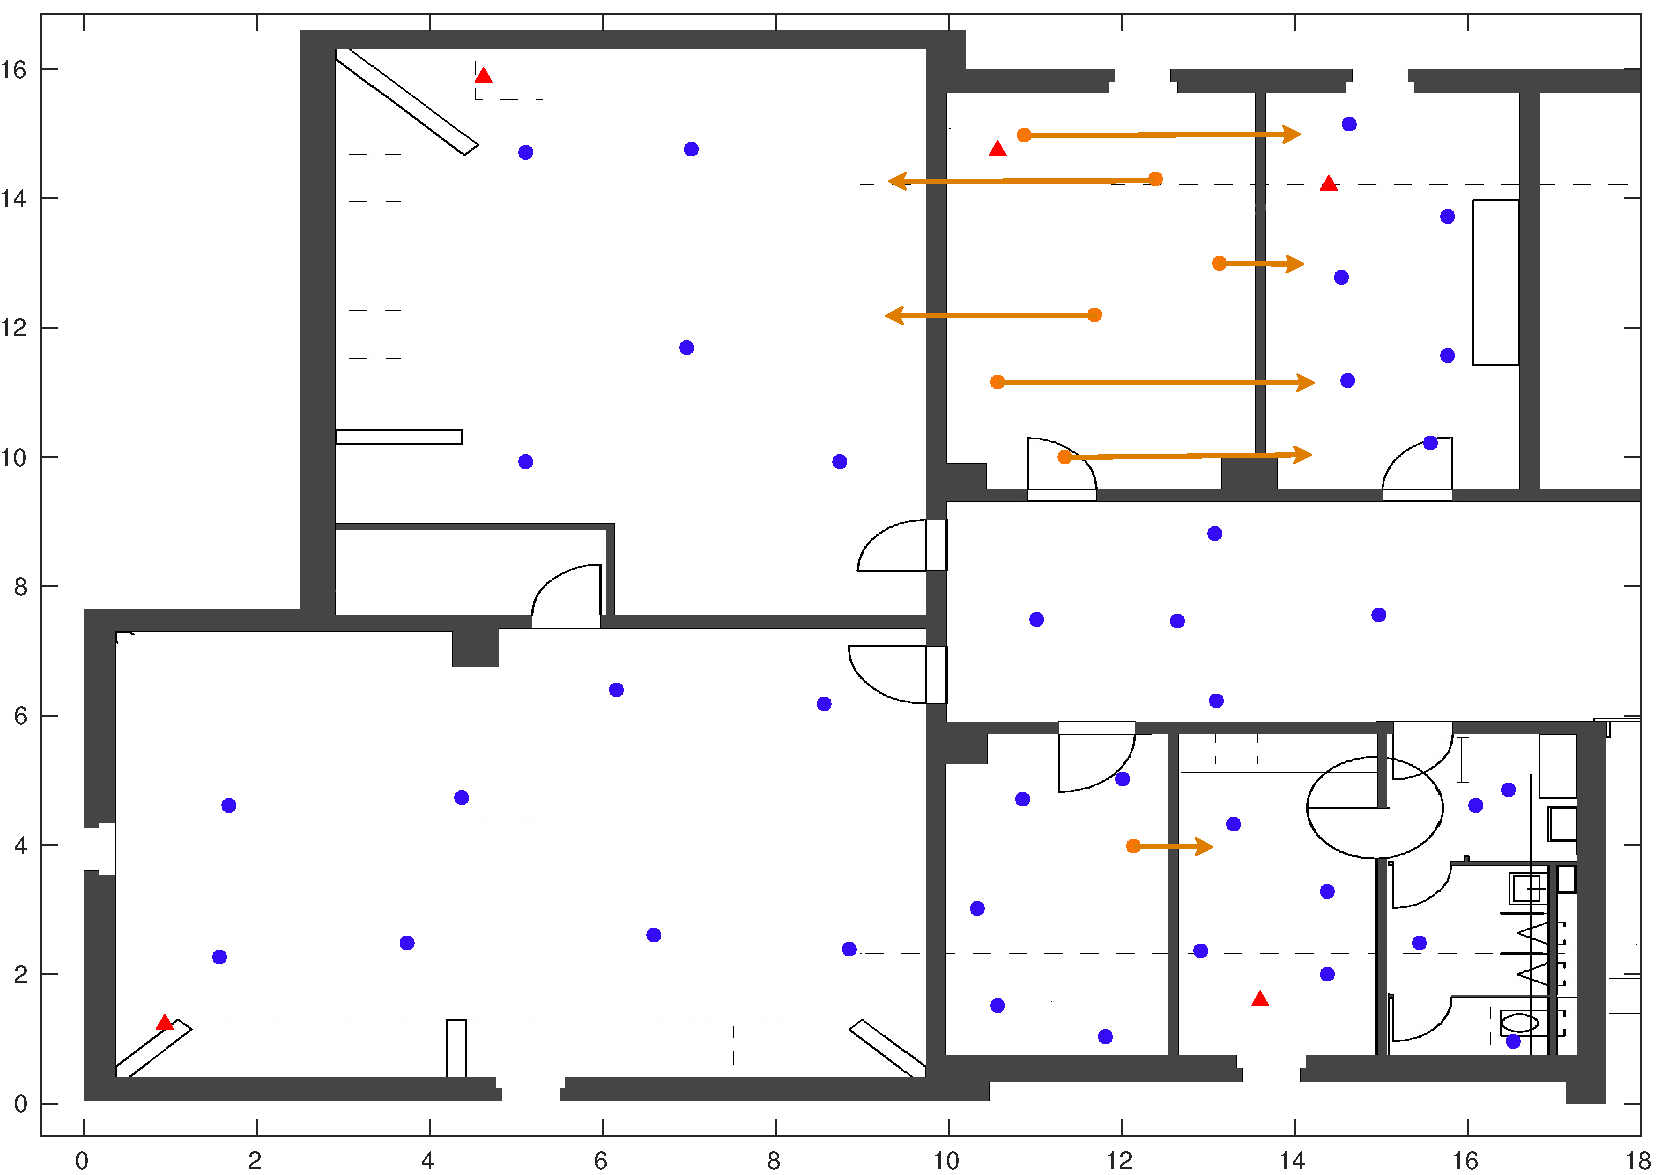
\includegraphics[width=.8\textwidth]{Figures/FloorPlan_Room_error_WithMF}
\decoRule
\caption[SVM kernel trick]{\raggedright(Left) A dataset in, not linearly separable. (Middle)The same dataset transformed with decision boundary. (Right) The nonlinear decision boundary.}

\end{figure}

Table \ref{tab:SVMconfigurationPresets} shows the accuracy for the different training data sets and two different kernel functions (pre-set parameters). The polynomial kernel performs very well while with the RBF kernel the accuracy is below 20\% for all training data sets. The RBF kernel, with these parameters, does not seem to be a good fit for this kind of data.

With the polynomial kernel the best performing data set is \emph{Borders+Center}, but it is only 2.3\% better than \emph{Grid}, which has 40\% fewer samples. This difference does not seem significant and is most likely due to the higher numbers of samples. \emph{Borders} has a pretty low accuracy in proportion to its numbers of samples. The accuracy of \emph{Center} is the lowest but still quite good considering it only has 66 samples. These results indicate that there is no benefit of having more samples at the borders.

Also the inclusion of magnetic field data improves the accuracy for all training sets except for the \emph{Borders+Center} data set. This is probably due to the parameters not being optimal (see Table \ref{tab:SVMconfigurationPoly}).

\begin{table}

\centering
\begin{tabular}{l l l l l}
\toprule
\textbf{Training Data}&\multicolumn{2}{c}{\textbf{Polynomial}}&\multicolumn{2}{c}{\textbf{RBF}}\\
\textbf{(\#Samples)}&\multicolumn{2}{c}{$c=1,e=1$}&\multicolumn{2}{c}{$c=1,g=0.01$}\\
&$RSSI_{i},B_{xyz}$&$RSSI_{i}$&$RSSI_{i},B_{xyz}$&$RSSI_{i}$\\
\midrule
Grid (223)&81.8\%&75\%&18.2\%&18.2\%\\
Center (66)&72.7\%&61.4&18.2\%&18.2\%\\
Borders (307)&77.3\%&65.9\%&13.7\%&13.7\%\\
Borders+Center (373)&84.1\%&84.1\%&11.4\%&11.4\%\\
\bottomrule
\end{tabular}
\caption[Room recognition - SVM pre-sets]{Accuracy of the room recognition with polynomial and RBF kernel pre-sets}
\label{tab:SVMconfigurationPresets}
\end{table}

Tables \ref{tab:SVMconfigurationRBF} and \ref{tab:SVMconfigurationPoly} show the accuracy with  optimal parameters for the polynomial and RBF kernel. For each training data set (with and without magnetic field data) and kernel function the optimal parameters were selected using grid search.

With the optimized parameters both kernels have a similar performance, although the RBF kernels $c$ values are generally higher. A high $c$ value means that the RBF kernel's decision surface needs to be more complex to achieve the same accuracy as the polynomial kernel. It is therefore not as good at separating the samples and polynomial kernel seems to be the better suited kernel function. 

For the training data sets the accuracy could be slightly increased by the parameter selection, but the distribution is still the same; The \emph{Borders+Center} has the highest performance with \emph{Grid} only being marginally worse, especially when reducing the number of samples in \emph{Borders+Grid} (see table \ref{tab:SVMconfigurationPoly}).

The magnetic field values again cause a improvement, although smaller than with the pre-sets.

\paragraph{To conclude the results of this experiment:} The inclusion of magnetic field data generally improves the room recognition accuracy. Although size of the improvement is dependent on the training data and the SVM's parameters.

The best performing training dataset, in comparison to the numbers of samples, is a \emph{evenly distributed Grid of samples}. 

The best suited kernel function is the polynomial kernel.



\begin{table}
\centering
\begin{tabular}{l l l l l l l}
\toprule
\textbf{Training Data}&\multicolumn{3}{c}{\boldmath$RSSI_{i},B_{xyz}$}&\multicolumn{3}{c}{\boldmath$RSSI_{i}$}\\
\textbf{(\#Samples)}&\textbf{accy}&$c$&$e$&\textbf{accy}&$c$&$e$\\
\midrule
Grid (223)&84.1\%&10&1&81.8\%&10&1\\
Center (66)&72.7\%&1&1&72.3\%&10&1\\
Borders (307)&84.1\%&10&1&77.3\%&10&1\\
Borders+Center (373)&88.6\%&100&1&86.4\%&10&1\\
Border+Center (223)&85.7\%&10&1&84.1\%&10&1\\
\multicolumn{7}{l}{\textit{40\% randomly removed, average of 10 evaluations}}\\
\bottomrule
\end{tabular}
\caption[Room Recognition - polynomial kernel parameter selection]{Results of the parameter selection for the polynomial kernel}
\label{tab:SVMconfigurationPoly}
\end{table}

\begin{table}
\centering
\begin{tabular}{l l l l l l l}
\toprule
\textbf{Training Data}&\multicolumn{3}{c}{\boldmath$RSSI_{i},B_{xyz}$}&\multicolumn{3}{c}{\boldmath$RSSI_{i}$}\\
\textbf{(\#Samples)}&\textbf{accy}&$c$&$g$&\textbf{accy}&$c$&$g$\\
\midrule
Grid (223)&84.1\%&100&0.01&81.8\%&1000&0.01\\
Center (66)&70.5\%&100&0.01&72.7\%&1000&0.01\\
Borders (307)&84.1\%&100&0.1&77.3\%&1000&0.01\\
Borders+Center (373)&86.4\%&1000&0.01&86.4\%&100&0.1\\
\bottomrule
\end{tabular}
\caption[Room Recognition - RBF kernel parameter selection]{Results of the parameter selection for the RBF kernel}
\label{tab:SVMconfigurationRBF}
\end{table}

\section{Weighting}
\label{EvaluationWeighting}

In Chapter \ref{WeightingModelDefinition} two weighting methods were proposed; the \emph{Room Weights} (equation \note{reference}) and the \emph{Room+Distance Weights} (equation \note{redrence}). The goal of this experiment is to evaluate if the \emph{Room Weights} improve the accuracy of the trilateration and if this is true whether the acuracy can be further improved with the \emph{Room+Distance Weights}.

During the training phase the \emph{ranging model} and the \emph{room weights} are trained with the entire \emph{XY} data set and imported into the trilateration tool. For evaluation the same data-set is used with the assumption of 100\% room recognition accuracy. The \emph{Distance Weights} are calculated during run time and combined with the \emph{Room Weights}.

\subsection{Results}
The results are presented as the cumulative distribution function of the localization error. This allows for a more accurate representation of the performance than just using statistical values like the mean and standard deviation.

The performance if the weighting methods is compared to \emph{Distance Weights} (equation \note{reference}) and \emph{ordinary least squares} (no weights).

\begin{figure}[htp]
\centering
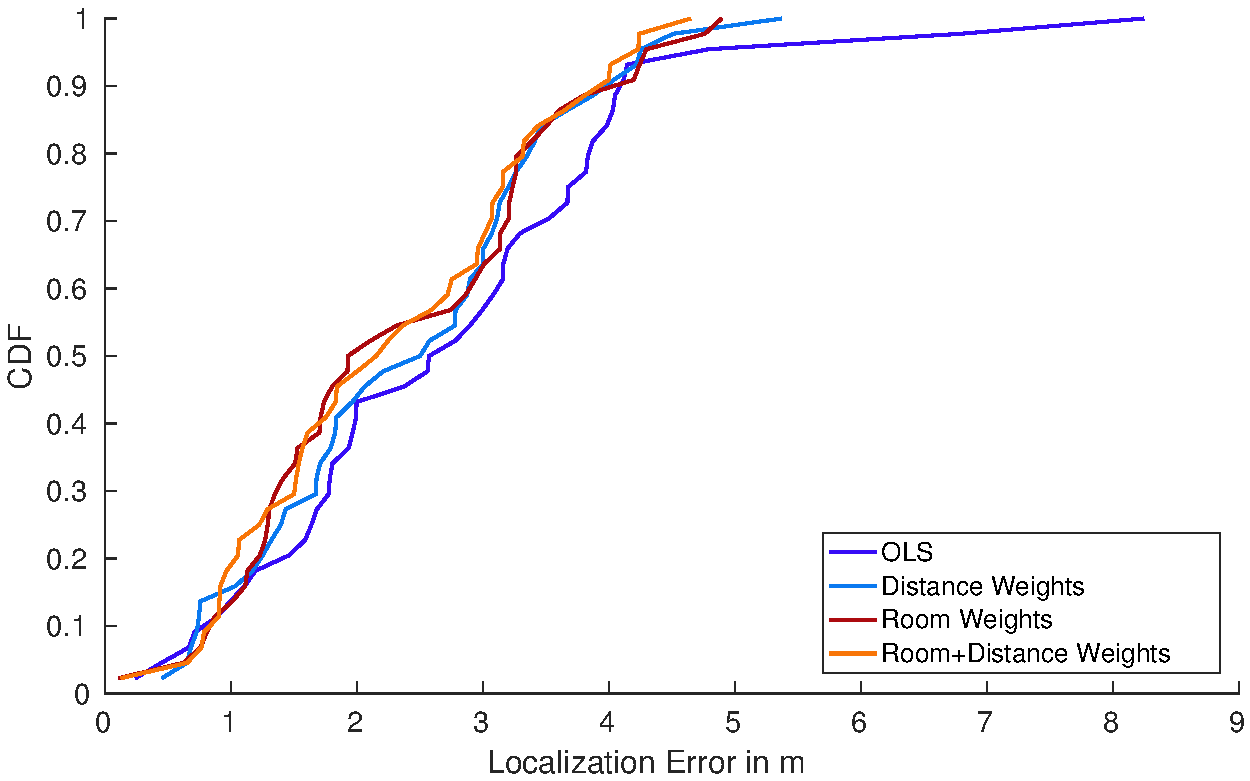
\includegraphics[width=\textwidth]{Figures/WeightingResultsCDF}
\decoRule
\caption[Weighting method comparison]{CDF of the Localization error for the different weighting methods.}
\label{fig:WeightingResultsCDF}
\end{figure}

\begin{table}
\centering
\begin{tabular}{l l l l l}
\toprule
\textbf{Weighting Method}&\textbf{Mean}&\textbf{Standard}&\textbf{Maximum}&\textbf{Improvement}\\
&&\textbf{Deviation}&\textbf{Error}&\textbf{over OLS}\\
\midrule
OLS&2.74m&1.57m&8.25m&\\
Distance Weights&2.42m&1.19m&5.37m&11.3\%\\
Room Weights&2.35m&1.22m&4.89m&14.2\%\\
Room+Distance Weights&2.29m&1.16m&4.65m&16.4\%\\
\bottomrule
\end{tabular}
\caption[Weighting method comparison]{Comparison of the statistical data for the different weighting methods}
\label{tab:WeightingStatisticalValues}
\end{table}

The results in figure \ref{fig:WeightingResultsCDF} and table \ref{tab:WeightingStatisticalValues} show a clear improvement of the \emph{Room Weights} over \emph{OLS}. The mean error is $\approx$0.4m lower, the standard deviation smaller and the maximum error was reduced by $\approx$3.4m. The difference is also clearly visible in the CDF plot.

But when compared to the \emph{Distance Weights} the improvements are much smaller. The mean error is only a few centimetres lower (0.07m) and at 70\% the \emph{Room Weights} are even a bit worse than the \emph{Distance Weights}. Here the largest improvement of the \emph{Room Weights} over the \emph{Distance Weights} is the maximum error, which was improved by $\approx$0.5m.

The results also show that Combining the \emph{Room} and \emph{Distance Weights} does indeed yield an improvement. While the mean error is only marginally increased, it lowers the maximum error even further and smooths out the CDF curve.

\paragraph{To conclude:} 

The proposed weighting methods work, offer good improvements over \emph{OLS} and greatly reduce the maximum error. They do, however, not perform much better than \emph{Distance Weights}.


\section{Final Evaluation}

For the final evaluation the room recognition and weighting are combined to evaluate the overall performance of the system. The results of the weighting experiment (previous section  \ref{ExperimentWeighting}) represent the maximum achievable accuracy under optimal conditions (100\% room recognition accuracy).  The main question for this evaluation is how much impact the room recognition error has on the localization accuracy.

The same training and testing set-up as in the weighting experiment was used.To see the impact of different room recognition accuracies on the weighting model, two room recognition models were used; one was trained with the \emph{Borders+Center} data set (88.6\% accuracy) and the other with the \emph{Grid} data set (84.1\%).

\subsection{Results}

The results are compared to the optimal case with 100\% room recognition accuracy and to the \emph{Distance Weights}.


\begin{table}
\centering
\begin{tabular}{l l l l l}
\toprule
\textbf{Weighting Method}&\textbf{Mean}&\textbf{Standard}&\textbf{Maximum}\\
&&\textbf{Deviation}&\textbf{Error}\\
\midrule
OLS&2.74m&1.57m&8.25m&\\
Distance Weights&2.42m&1.19m&5.37m&11.3\%\\
Room+Distance Weights (100\%)&2.29m&1.16m&4.65m&16.4\%\\
Room+Distance Weights (84.1\%)&2.40m&1.25m&5.69m&12.4\%\\
\bottomrule
\end{tabular}
\caption[Final evaluation statistical values]{Comparison of the statistical data for the final evaluation}
\label{tab:FinalStatisticalValues}
\end{table}